\section{Compilations into Goal Dependencies}

\rebecca{ 1-1.5 page(s) Michael/Rebecca }

\rebecca{Define a FDR task}

\subsection{Action Set Compilation}

\joerg{there first needs to be a separate definition of
  \defined{action constraints}. Then a definition similar to the one
  below, that specifies the compilation. Then a formal Proposition
  claiming that the compilation is correct: given task \task\ with
  induced plan set \plans\ and plan property set \props\ consisting of
  goal facts and action constraints, if \task', \plans', and \props'
  is the compiled task, induced plan set, and property set, then a PDA
  for \plans\ and \props\ can be constructed in polynomial time from
  one for \plans' and \props'. In the final paper, the proof can be a
  short textual explanation, not in a formal proof environment,
  basically just describing how to do this and why it works; but
  please first make a more formal detailed proof that explicitly gives
  the polynomial time algorithm and argues in detail why indeed the
  result is a PDA for \plans\ and \props.}

The plan properties \textit{"Only one truck is used."} or \textit{"Package A and 
B are delivered by the same truck"} restrict the actions which can be used to 
achieve a goal. To include properties in our framework which are described by a
propositional logic with the atoms \emph{plan uses at least one action from $A_i$} 
where $A_i \subset A$, we introduce a compilation from such expressions.

\begin{definition}
	Let $\Pi = (V, A, c, I)$ be the original planning task and $A_P=\{A_0, \cdots, A_n\}$ 
	a partition of $A$ \joerg{does it really have to be a partition? and does that restriction make sense? I think neither is the case: in the compilation, a single action could set several flags, one for each action set it belongs to; and certainly one can think of constraints where the relevant action sets overlap} and a propositional formal $\mathcal{P}$ over the atoms $\mathcal{F} = \{f_i | A_i \in A_p\}$. 
	Then the action set compilation $\Pi' = (V', A', c, I')$ is defined as: 
	$V' = V \cup \{\text{used}_i | A_i \in A_P\} \cup \{\text{sat}_{\mathcal{P}}, \text{eval-phase}\}$ 
	with $\mathcal{D}_{\text{used}_i} = \mathcal{D}_{\text{sat}_{\mathcal{P}}} = \mathcal{D}_{\text{eval-phase}} = \{0,1\}$, 
	$I' = I \cup \{\text{used}_i = 0 | A_i \in A_P\} \cup \{\text{sat}_{P} = 0, \text{eval-phase} = 0\}$ 
	and $A' = \{ a' | a \in A, 
	\text{pre}_{a'} = \text{pre}_{a} \cup \{\text{eval-phase} = 0\} \text{eff}_{a'} = \text{eff}_a \cup 
	\{\text{cp} | \text{pre}_{cp} = \{\text{eval-phase} = 0\}, \text{eff} = \{\text{eval-phase} = 1 \}\} \cup 	
	\{\text{used}_i = 1 | a \in A_i \in A_P\} \cup  
	\{\text{actions to eval } \mathcal{P}\}$. 
\end{definition}

\rebecca{how to define the eval actions}

For every action set $A_i$ in $A_P$ we introduce a new fact $\text{used}_i$ which is initially 
\emph{false} and changed to \emph{true} by any action in $A_i$. The new variable $sat_{\mathcal{P}}$ indicates 
if the property $\mathcal{P}$ is satisfied at the end of the plan. To prevent an 
evaluation of the property before the end of the plan we introduce an additional binary variable
which indicates if we are in the execution or evaluation phase of the action sequence. Once the \textit{change-phase} (cp) action
is applied no original actions can be executed anymore and the actions sequence is evaluated.

\rebecca{
	ideally you would add the goal facts to the \emph{change-phase} action to force a switch to the 
	evaluation phase after all goals are achieved. This is not compatible with the search for the goal fact 
	dependencies. You have to adapted the precondition of the action according to the current goal subset. 
	(is possible but it is not clear to me if you can still reuse the heuristic for different subsets) 
}


\paragraph{Example} If we choose $A_P = \{A_1, A_2\}$ were $A_i$ contains all actions where truck $i$ 
is involved, we can express the property \emph{"Only one truck is used"} with the 
formula $(u_1 \wedge \neg u_2) \vee (\neg u_1 \wedge u_2)$.

\subsection{LTL}

\rebecca{the compilation of Edelkamp can be used out of the box. If you want to compile multiple properties at 
	the same same time into the planning task (e.g. for the goal dependencies check) you have to use \emph{complete} 
	Büchi automate. Otherwise it is possible that a property influences the result by causing a deadend even if the corresponding
	goal fact it not considered
}

	Example: Package 0 is never in truck 1. $\square ! \text{in}(P_0,T_1)$

	\begin{minipage}{0.22\textwidth}
		\centering
		\tiny
		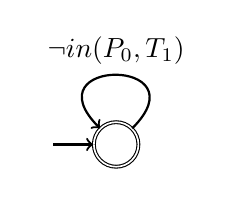
\begin{tikzpicture}
			\node[draw, circle, inner sep=0.2cm, double] (i) at (0,0) {};
			\draw[->, thick, loop] (i) to node[above] {$\neg \text{in}(P_0,T_1)$}(i); 
			\draw[->, thick] (-0.8,0) to (i); 
		\end{tikzpicture}
	\end{minipage}
	\hfill
	\begin{minipage}{0.22\textwidth}
		\centering
		complete \\
		\tiny
		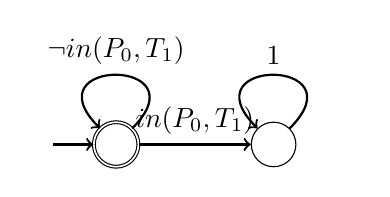
\begin{tikzpicture}
			\node[draw, circle, inner sep=0.2cm, double] (i) at (0,0) {};
			\node[draw, circle, inner sep=0.2cm] (d) at (2,0) {};
			\draw[->, thick, loop] (i) to node[above] {$\neg \text{in}(P_0,T_1)$} (i); 
			\draw[->, thick] (i) to node[above] {$\text{in}(P_0,T_1)$} (d);
			\draw[->, thick, loop] (d) to node[above] {$1$} (d); 
			\draw[->, thick] (-0.8,0) to (i); 
		\end{tikzpicture}
	\end{minipage}

\rebecca{the left automate creates a deadend in the compilation if $P_0$ is not in $T_1$ while the right does not.} 
